\documentclass[tikz]{standalone}

\usetikzlibrary{positioning}

\newcommand{\distro}[4][40]{
  \begin{tikzpicture}[thick]
    \draw[dashed, dash pattern={on 2.3 off 2}] (0, .4) circle (12mm);
    \draw[blue!60!black, very thick] plot[variable=\t, domain=-1:1, samples=#1] ({\t}, {#2 * exp(-10*(\t)^2) + #3 * exp(-60*(\t-0.6)^2 - \t) + #3 * exp(-60*(\t+0.7)^2 - 0.2) + #4 * 0.5 * exp(-50*(\t+0.3)^2) + #4 * exp(-50*(\t-0.2)^2 + 0.1)});
    \draw[solid, ->] (-1, 0)--(1, 0);
    \draw[solid, ->] (0, -0.5)--(0, 1.25);
  \end{tikzpicture}
}

\begin{document}
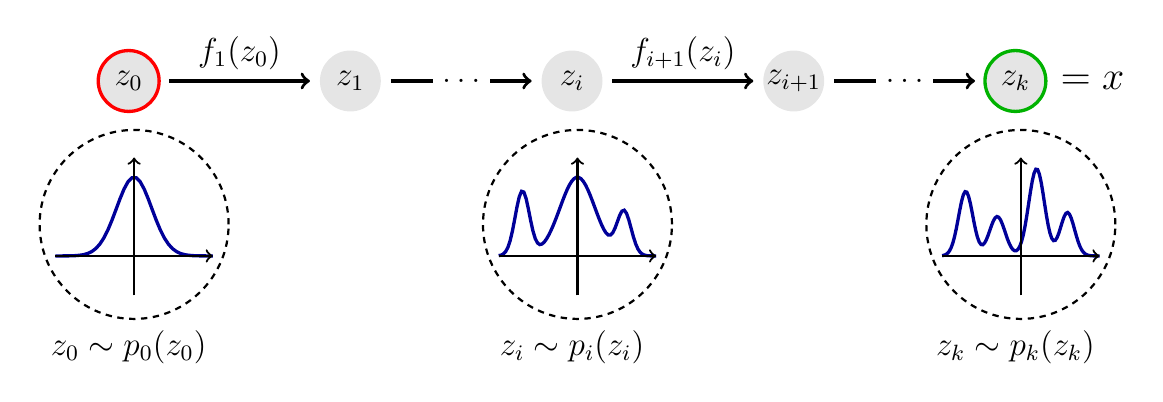
\begin{tikzpicture}[
    node distance=2, very thick, font=\large,
    flow/.style={shorten >=3, shorten <=3, ->},
    znode/.style={circle, fill=black!10, minimum size=22, inner sep=0},
  ]

  \node[znode, draw=red] (z0) {$z_0$};
  \node[znode, right=of z0] (z1) {$z_1$};
  \draw[flow] (z0) -- node[above, midway] {$f_1(z_0)$} (z1);

  \node[znode, right=of z1] (zi) {$z_i$};
  \node[znode, right=of zi] (zip1) {$z_{i+1}$};
  \draw[flow] (zi) -- node[above, midway] {$f_{i+1}(z_i)$} (zip1);
  \draw[flow] (z1) --node[rectangle, fill=white, anchor=center, midway] {$\dots$} (zi);

  \node[znode, draw=green!70!black, right=of zip1] (zk) {$z_k$};
  \draw[flow] (zip1) -- node[rectangle, fill=white, anchor=center, midway] {$\dots$} (zk);
  \node[right=0 of zk, scale=1.2] {$= x$};
  \node[outer sep=0, inner sep=0, below=0.2 of z0, label={below:$z_0 \sim p_0(z_0)$}] (f0) {\distro{1}{0}{0}};
  \node[outer sep=0, inner sep=0, below=0.2 of zi, label={below:$z_i \sim p_i(z_i)$}] (fi) {\distro[70]{1}{1}{0}};
  \node[outer sep=0, inner sep=0, below=0.2 of zk, label={below:$z_k \sim p_k(z_k)$}] (fk) {\distro[90]{0}{1}{1}};

\end{tikzpicture}
\end{document}